\documentclass[10pt,a4paper]{report}
\usepackage[utf8]{inputenc}
\usepackage[english]{babel}
\usepackage{amsmath}
\usepackage{amsfonts}
\usepackage{amssymb}
\usepackage{graphicx}
\usepackage{float}
\usepackage{hyperref}
\usepackage[autostyle, italian=quotes]{csquotes}
\usepackage[left=2cm,right=2cm,top=2cm,bottom=2cm]{geometry}
\author{Daniele Gilio}
\title{Spoken Digits Recognition}
\begin{document}
\maketitle
\section{Introduction}
This assignment is about spoken digits recognition. The dataset is comprised of $1760$ training samples, $120$ validation samples and $120$ test samples. The dataset has already been processed so that each sample represents the spectrogram of a given digit. Spectrograms are visual representation of audio files, the power of the recorded sound wave is divided between $16$ frequencies and $64$ time periods creating images like the one in Figure \ref{fig:data_spect}. Our objective is to create a Neural Network (a Multi-Layer Perceptron to be precise) in order to recognize the spoken digits.
\begin{figure}[!ht]
\centering
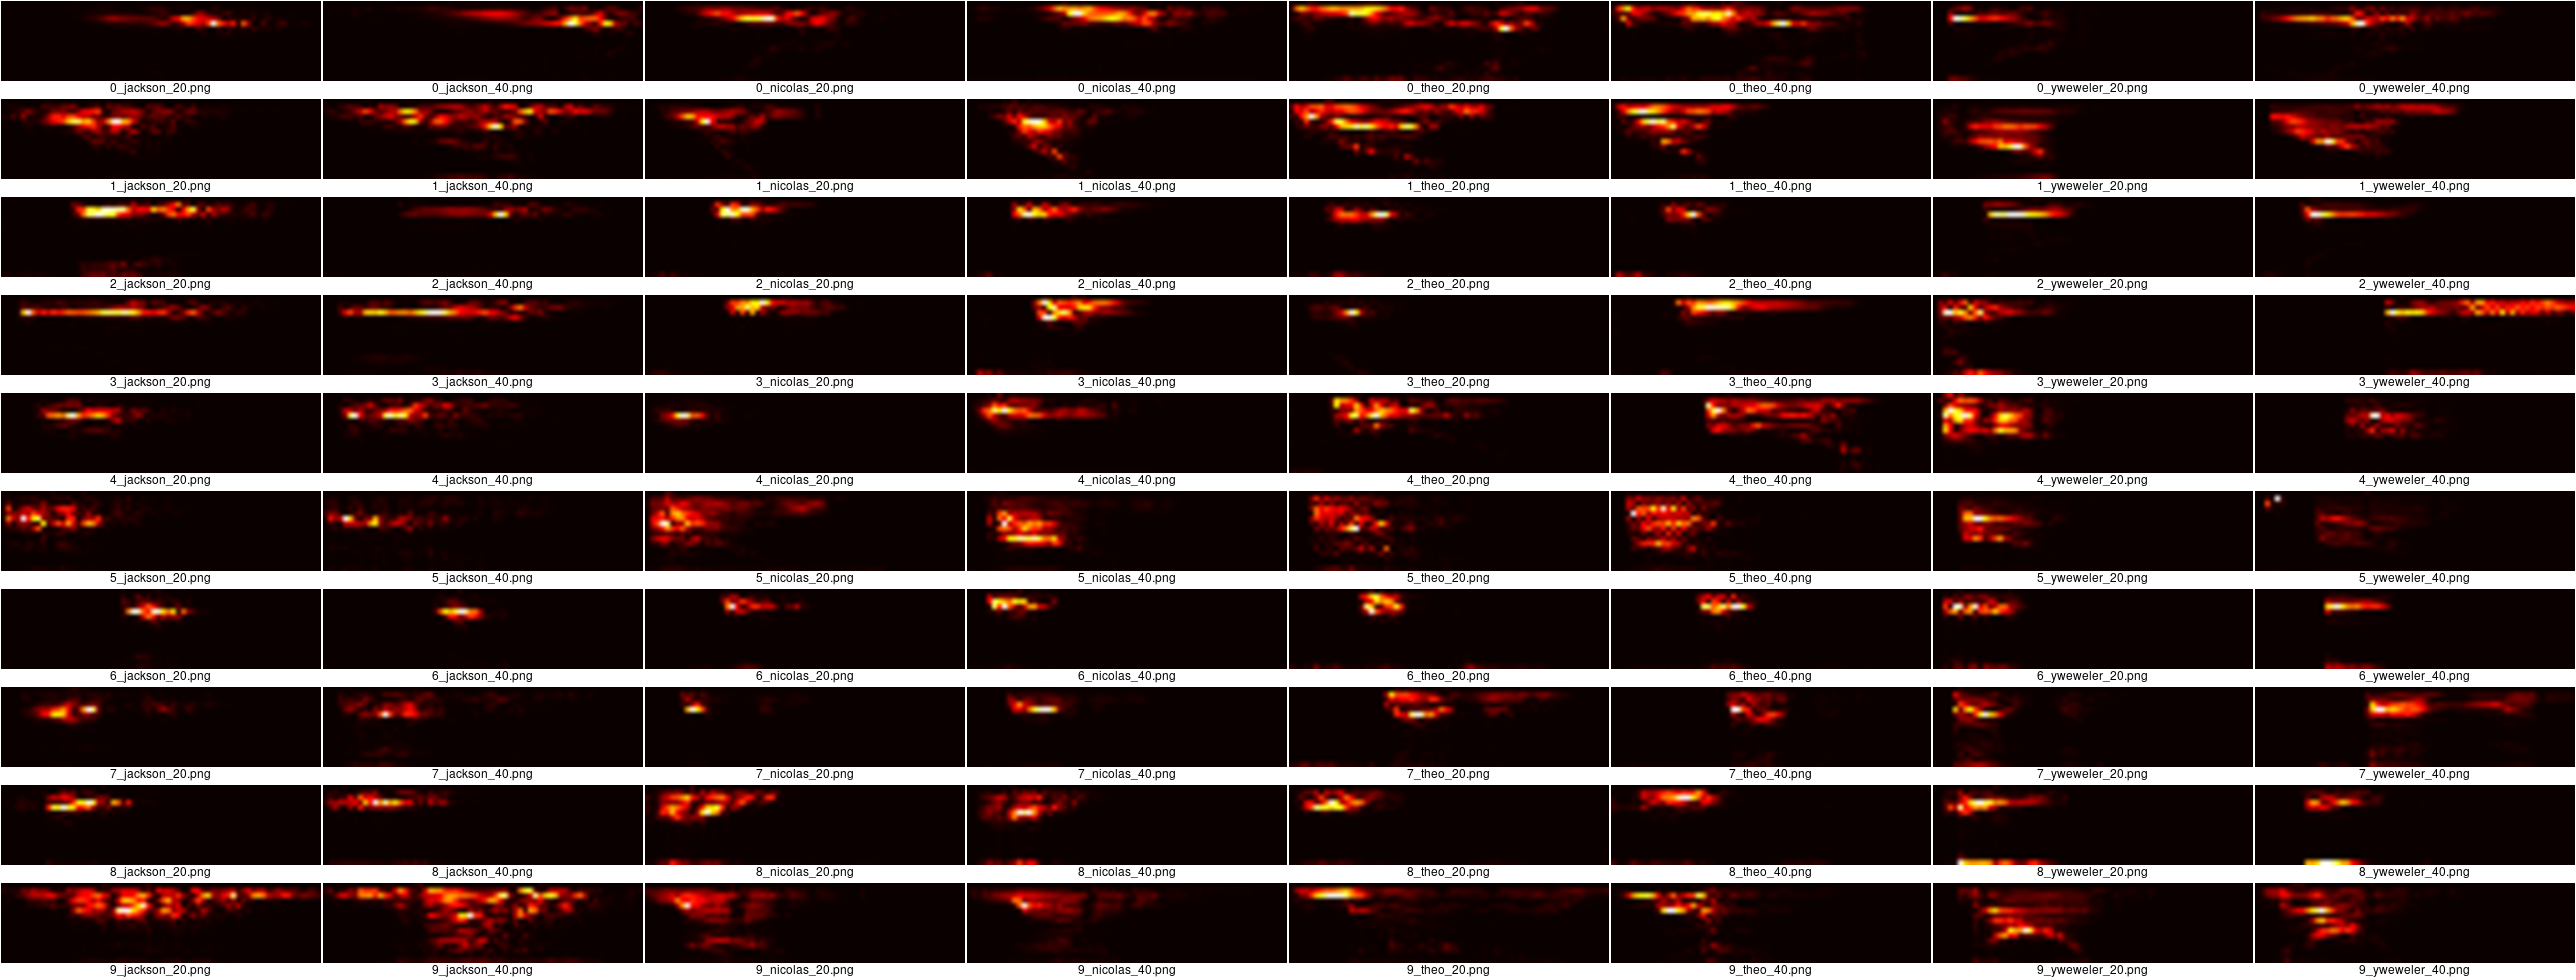
\includegraphics[width=\linewidth]{spoken-digits/spectrograms.png}
\caption{Example of the dataset spectrograms}
\label{fig:data_spect}
\end{figure}
\section{Data Visualization and Analysis}
In order to test our code we plotted spectrograms after we loaded the data and after performing normalization. The second plotting was also done in order to verify that the normalization did not interfere too much with the data. At this stage we opted for a Mean-Variance Normalization since it is the most common and we do not believe that the dataset geometry would be hugely altered. We can see the output of our code in Figure \ref{fig:norm_spect}.
\begin{figure}[!ht]
\centering
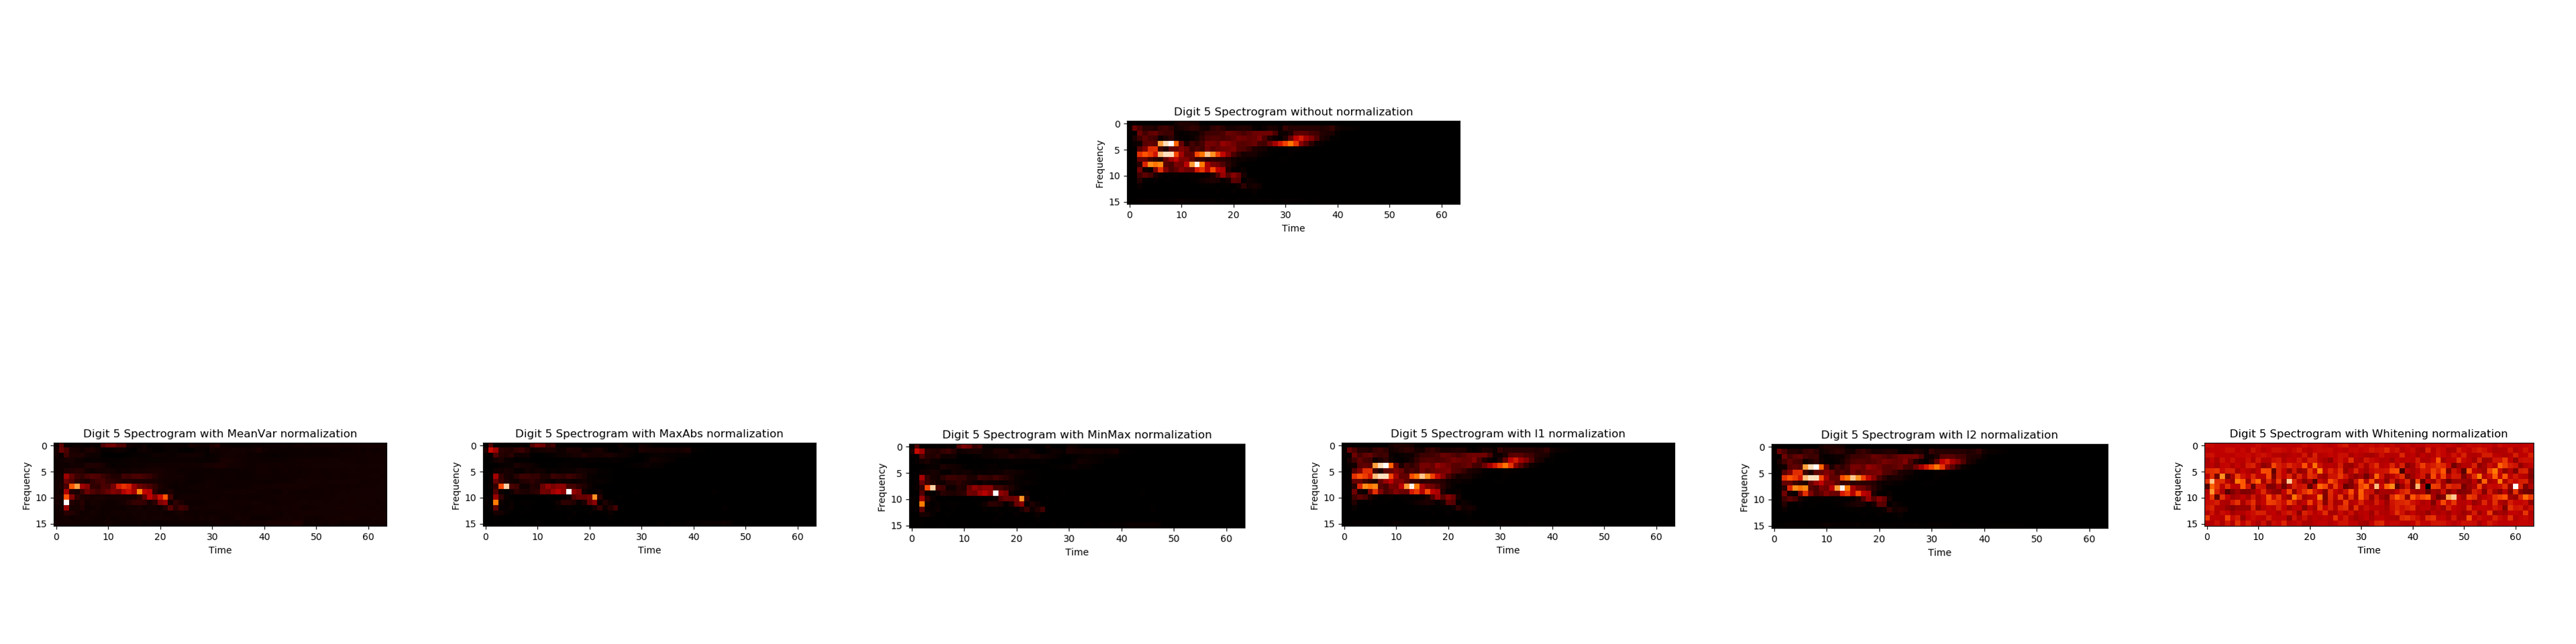
\includegraphics[width=\linewidth]{norm_spect.png}
\caption{Original Spectrogram (Top) and Normalized Spectrograms (Bottom)}
\label{fig:norm_spect}
\end{figure}
\section{Neural Network}
In order to experiment a bit with Neural Networks we built a Single-Layer Perceptron in which we have only an input layer and an output layer. As in the previous assignment we implemented a varying learning rate.
\subsection{Architecture}
After playing a bit with network architectures we settled on the following sequence $[1024, 256, 128, 32, 10]$, representing the width of each layer. Bigger models tended to overfit and took a long time to train, on the other hand tinier models were faster to train but less precise. We believe that optimal values are not very far from the ones we found.
\subsection{Hyperparameters and Training}
In order to train our network we tested Gradient Descent, SGD and mini-batch SGD. The first one proved to be the smoothest but the slowest and hardware demanding, SGD was the fastest but the most erratic. Mini-batch SGD was a good compromise between the two. We obtained the best results with a batch size of $8$ for the Single-Layer Network and a size of $256$ for the Multi-Layer one. The number of steps was adjusted accordingly to the batch size, so that $\textit{batch\_size} \cdot \textit{steps} \simeq \textit{training\_samples}$. Both networks were trained for $1000$ epochs to ensure they reached convergence. The starting learning rate was set at $0.01$, the regularization coefficient and the momentum coefficient were left untouched, respectively at $10^{-5}$ and $0.99$. 
\subsection{Normalization Techniques}
We decided to further investigate normalization techniques and to do that we performed a training for each one. We noticed that the batch size is very impactful on this test, small batch sizes tend to favor L2 Regularization whereas bigger batch sizes favor MeanVar Normalization. We can see a plot of all the test performed on the Multi-Layer Network (with the hyperparameters listed before) in Figure \ref{fig:norm_test}.
\begin{figure}[!ht]
\centering
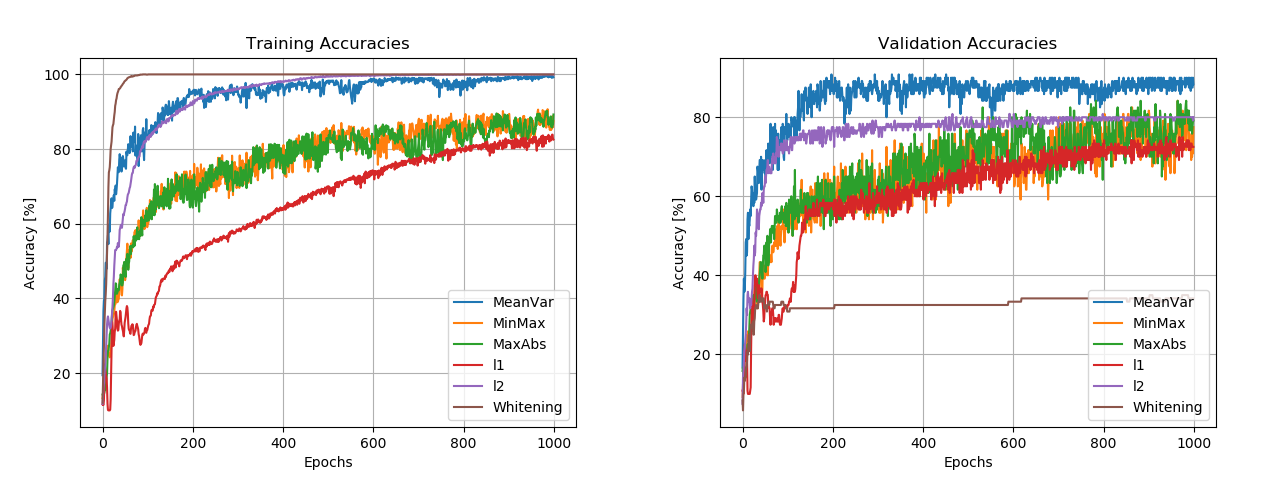
\includegraphics[width=\linewidth]{accs.png}
\caption{Training Accuracies (Left) and Validation Accuracies (Right)}
\label{fig:norm_test}
\end{figure}
From the data we collected we can say that MeanVar is the best overall performer, whereas Whitening is the worst. There is no clear separation between instance normalizations and statistical based ones since L2 normalization is the second most performing normalization.  
\section{Results}
The final predictions on the test set reached a percentage between $87.5$ and $90$ for the Multi-Layer Network and between $69$ and $72$ for the Single-Layer one. We can take a look at the \textit{Confusion Matrix} to better see how the networks perform. Examining the confusion matrices in Figure \ref{fig:conf_mat}, we can see that the Multi-Layer Network performs better as expected. We can also see that the most incorrect predictions were given for digits $0$ and $3$ in the case of the Single-Layer Network and $1$ and $3$ for the Multi-Layer. 
\begin{figure}[H]
\centering
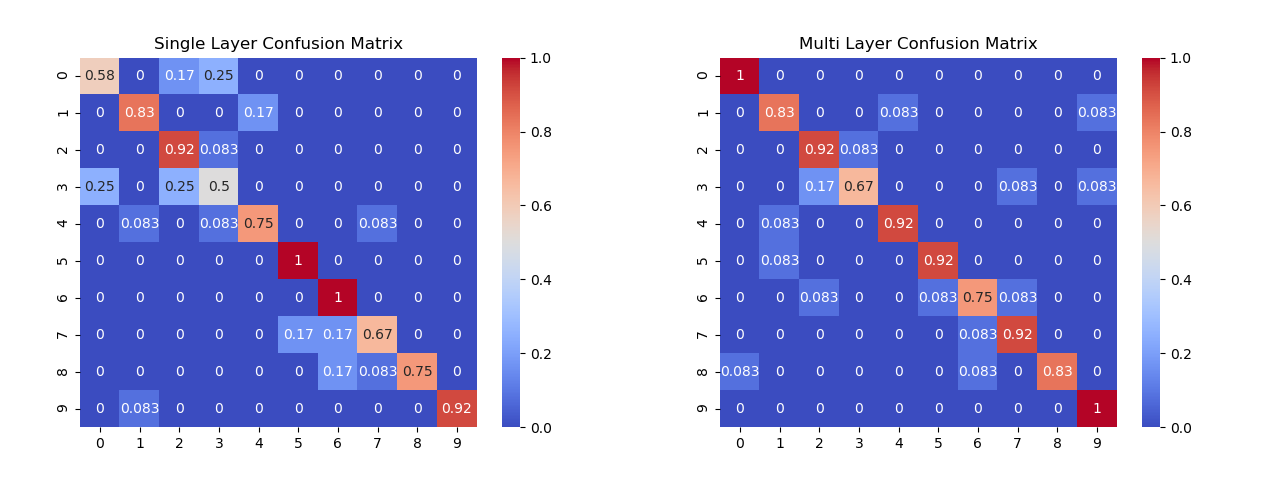
\includegraphics[width=0.8\linewidth]{conf_mat.png}
\caption{Single Layer (Left) and Multi Layer (Right) Confusion Matrices}
\label{fig:conf_mat}
\end{figure}
With regards to the Single-Layer Network we can also take a look at the weights, which should represent the spectrograms used by the network to make predictions. In Figure \ref{fig:nn_spect} we see that $0$ and $3$ have very similar spectrograms as we expected from the confusion matrix. The Single Layer Network mostly uses the fist part of the spectrogram, commonly called the \enquote{\textit{attack}}. It also uses the \enquote{\textit{tail}} for the $0$ which has a very distinct one. In the Multi-Layer case a direct weight interpretation is very difficult but we can manually listen to the samples which are misclassified with the most confidence. Some of them are perfectly discernible for a human while others can be a bit tricky since we feel that the signal-to-noise ratio is probably low.
\begin{figure}[H]
\centering
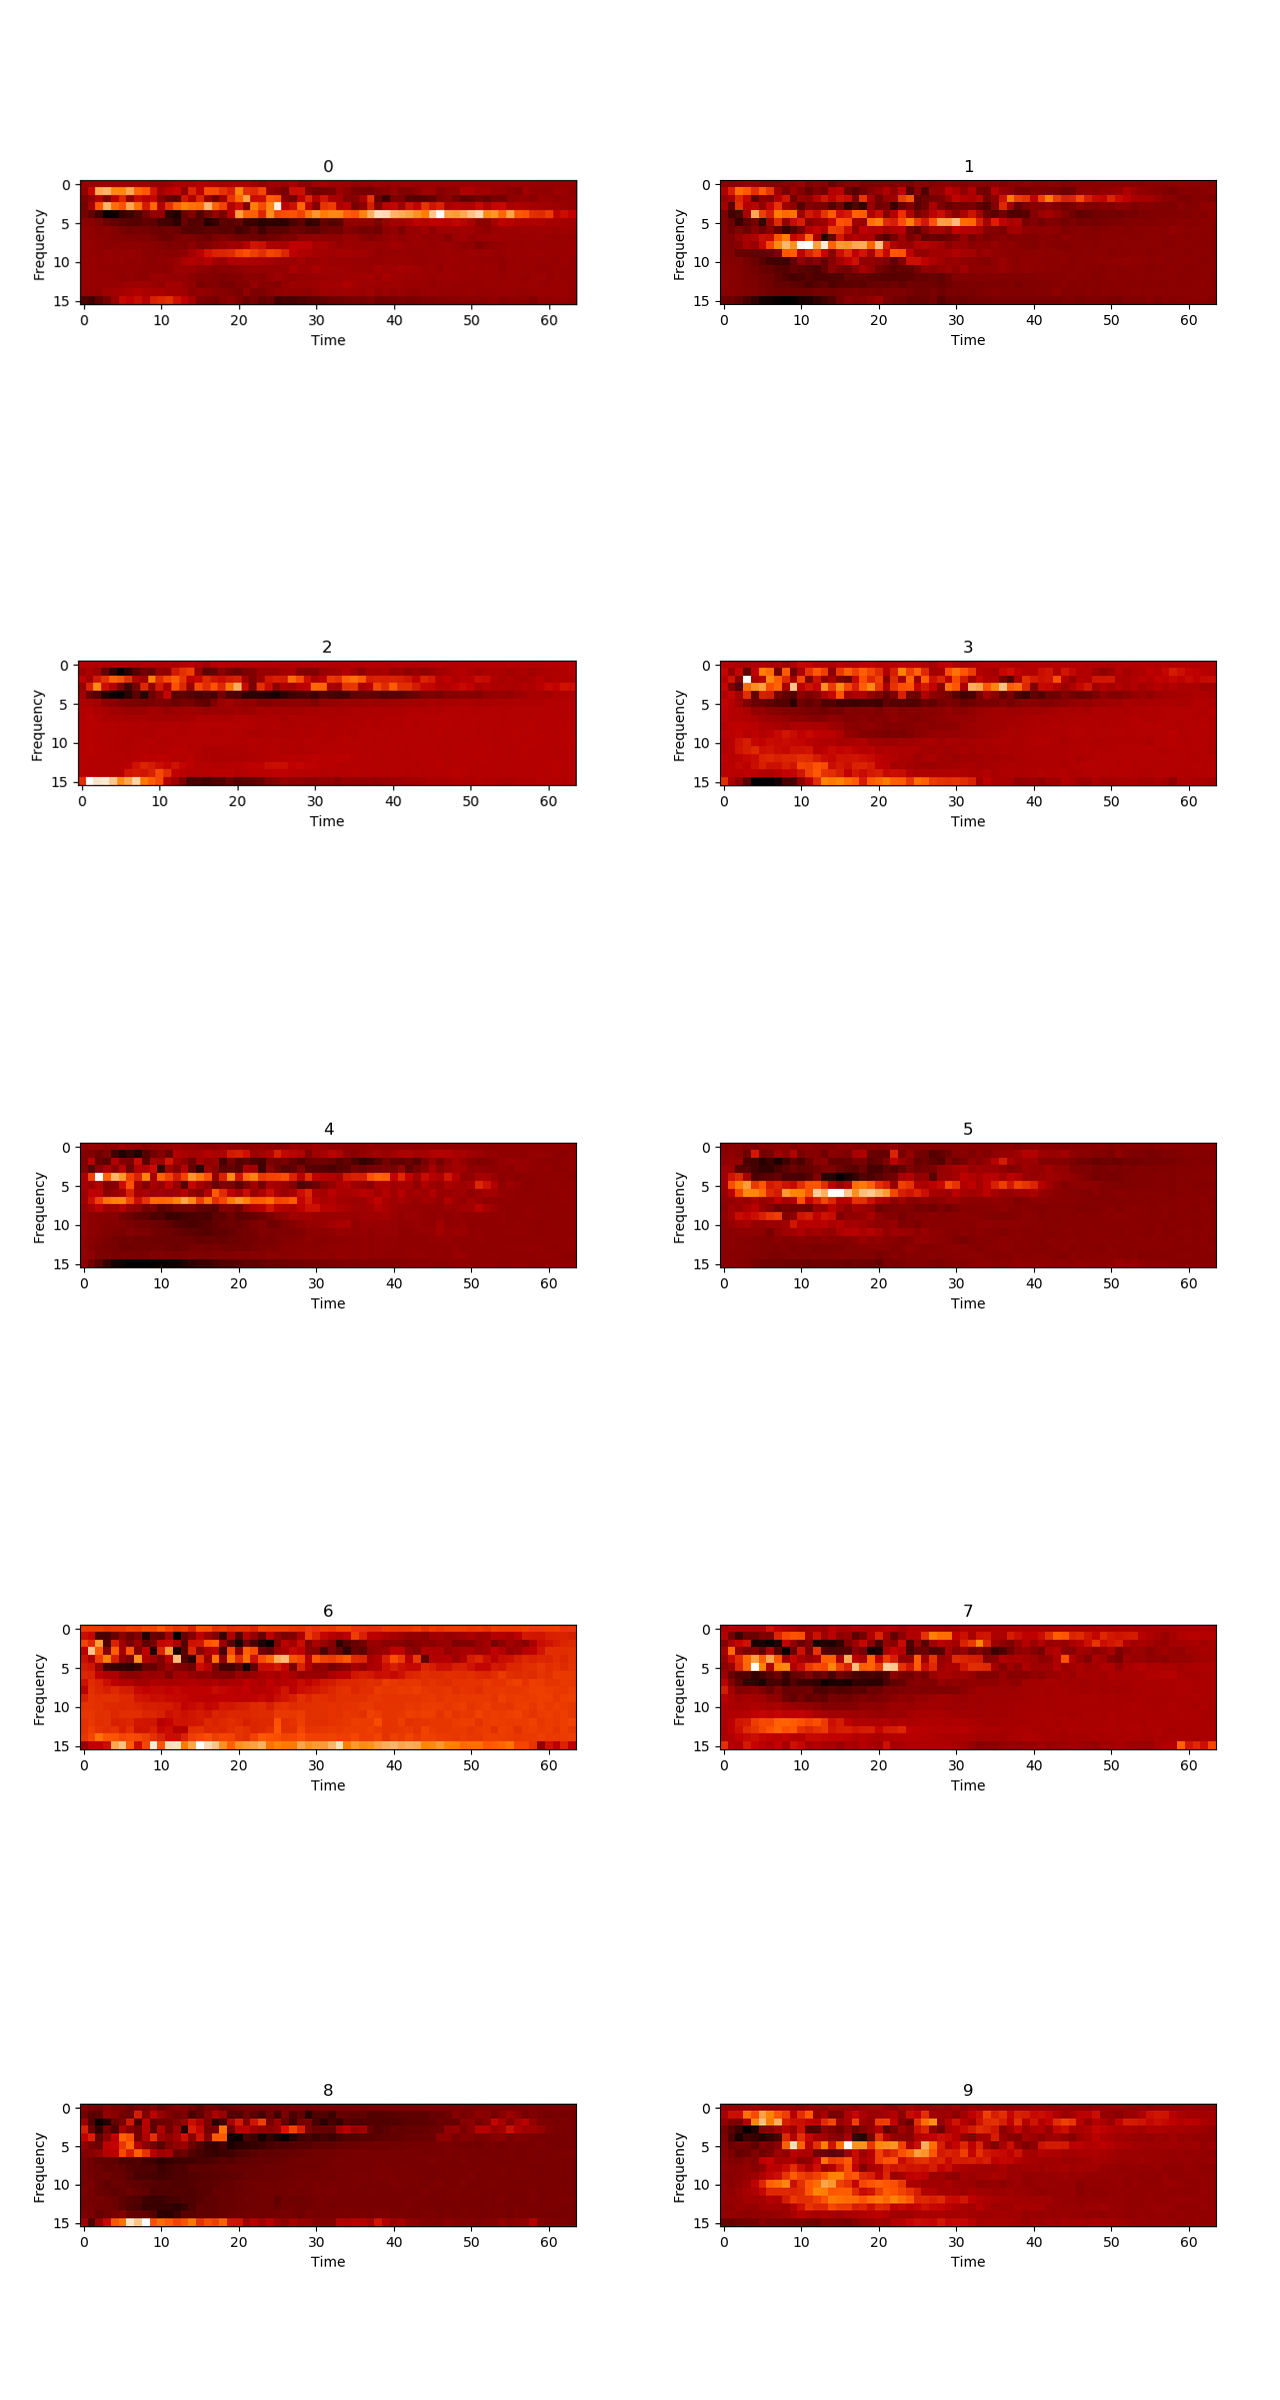
\includegraphics[scale=0.12]{nn_spec.png}
\caption{Single Layer Network Weights}
\label{fig:nn_spect}
\end{figure}
\section{Conclusions}
In conclusion we can say that the Multi Layer Perceptron is a better choice for this particular classification problem. The Single Layer Perceptron is a good first try but its linearity limits its capabilities significantly. Introducing some kind of memory in the neurons might help improving the network performance, since each instance in the feature vectors is strongly correlated to the ones around it, being a representation of an audio file. One could also think about improving the time resolution of the spectrograms in order to give the networks more information to learn from. As always expanding the dataset would also be a good idea, $1760$ training samples are kind of on the tiny dataset side. That said our Multi Layer Network works quite well given the context.
\vspace*{\fill}
\\
I affirm that this report is the result of my own work and that I did not share any part of it with anyone else except the teacher.
\\ \\ 
\end{document}